\section{Présentation}

%%%%%%%%%%%%%%%%%%%%%%%%%%%%%%%%%%%%%%%%%%%%%%%%%%%%%%%%%%%%%%%%%%%%%%%%%%%%%%%%

\begin{frame}[fragile]{Histoire brève de PostgreSQL - POSTGRES}

   \begin{itemize}
      \item PostgreSQL est dérivé du projet POSTGRES amorcé par l'Université de Californie à Berkeley
      \item POSTGRES est né en 1986 et a été financé par:
      \begin{itemize}
         \item le DARPA (Defense Advanced Research Projects Agency)
         \item l'ARO (Army Research Office)
         \item le NSF (National Science Foundation)
         \item ESL Inc.
      \end{itemize}
      \item POSTGRES a été utilisé par différents projets universitaires.
      \item Illustra Information Technologies qui a fusionné avec Informix, rachetée par IBM commercialise le code dans les années 90
   \end{itemize}

\begin{toile}
\toileurl{https://www.postgresql.org/docs/15/history.html}
\end{toile}

\end{frame}

%%%%%%%%%%%%%%%%%%%%%%%%%%%%%%%%%%%%%%%%%%%%%%%%%%%%%%%%%%%%%%%%%%%%%%%%%%%%%%%%

\begin{frame}[fragile]{Postgres95}

   \begin{itemize}
      \item En 1993, la communauté d'utilisateurs double de taille.
      \item La maintenance du projet devient très chronophage pour les équipes de recherche universitaires qui décident de mettre fin au projet avec la publication finale de la version 4.2
      \item En 1994, Andrew Yu et Jolly Chen ajoutent un interpréteur SQL à POSTGRES
      \item Le projet change de nom pour devenir Postgres95, l'héritier open source de POSTGRES
      \item Postgres95 est entièrement écrit en ANSI C et son code est réduit de 25\%.
      \item Postgres95 v1.0 est 30-50\% plus rapide que POSTGRES
   \end{itemize}

\end{frame}

%%%%%%%%%%%%%%%%%%%%%%%%%%%%%%%%%%%%%%%%%%%%%%%%%%%%%%%%%%%%%%%%%%%%%%%%%%%%%%%%

\begin{frame}[fragile]{PostgreSQL}

   \begin{itemize}
      \item Le langage PostQUEL est définitivement abandonné au profit de SQL
      \item Le client psql est développé. Il utilise la librairie GNU readline
      \item Le support des grands objets (Large Objects) est mis en place
      \item En 1996, Postgres95 devient PostgreSQL car il semble important que l'année ne figure pas dans le nom
      \item Il est aussi possible de l'appeler Postgres (en référence à son ancêtre)
   \end{itemize}

\end{frame}

%%%%%%%%%%%%%%%%%%%%%%%%%%%%%%%%%%%%%%%%%%%%%%%%%%%%%%%%%%%%%%%%%%%%%%%%%%%%%%%%

\begin{frame}[fragile]{Exercice - Installer PostgreSQL 15 sur les serveurs de formation}

   \begin{itemize}
      \item Installer le serveur PostgreSQL sur les serveurs \textbf{hqpg-0x} et \textbf{hqpg-0x-repl}
      \item Les serveurs ont pour OS Rocky Linux version 8
   \end{itemize}

\begin{toile}
\toileurl{https://www.postgresql.org/download/linux/redhat/}
\toileurl{https://rockylinux.org/}
\end{toile}

\end{frame}

%%%%%%%%%%%%%%%%%%%%%%%%%%%%%%%%%%%%%%%%%%%%%%%%%%%%%%%%%%%%%%%%%%%%%%%%%%%%%%%%

\section{Ecosystème}

\begin{frame}{Présentation de l'écosystème PostgreSQL}

   \begin{itemize}
      \item La communauté PostgreSQL met à disposition un nombre assez important d'outils pour faciliter la vie des utilisateurs et des administrateurs
      \item Les outils suivants vont être présentées durant cette formation:
      \begin{itemize}
         \item POWA
         \item pgBadger
         \item pgAdmin4
      \end{itemize}
   \end{itemize}


\end{frame}

%%%%%%%%%%%%%%%%%%%%%%%%%%%%%%%%%%%%%%%%%%%%%%%%%%%%%%%%%%%%%%%%%%%%%%%%%%%%%%%%

\begin{frame}{POWA}

   \begin{itemize}
      \item PoWA signifie "PostgreSQL Workload Analyzer"
      \item Il supporte PostgreSQL 9.4+
      \item PoWA permet de collecter, agréger et purger des statistiques sur plusieurs instances PostgreSQL depuis plusieurs extensions statistiques
      \item En fonction des besoins de l'utilisateur, PoWA fonctionne avec 2 modes:
   \begin{itemize}
         \item en utilisant le \textbf{background worker}. Ce fonctionnement est adapté aux environnements mono instances. Il nécessite un redémarrage de la base.
         \item en utilisant le \textbf{PoWA collector}. Ne nécessite pas de redémarrage, collecte les informations depuis plusieurs bases, le standby inclus
   \end{itemize}

   \end{itemize}

\begin{tiny}
\begin{toile}
\toileurl{https://powa.readthedocs.io/en/latest/}
\end{toile}
\end{tiny}

\end{frame}

%%%%%%%%%%%%%%%%%%%%%%%%%%%%%%%%%%%%%%%%%%%%%%%%%%%%%%%%%%%%%%%%%%%%%%%%%%%%%%%%

\begin{frame}{POWA - modules de statistiques}

   \begin{itemize}
      \item Les modules de statistiques supportés par PoWA sont:
      \begin{itemize}
         \item \textbf{pg\_stat\_statements} fournit des informations sur les requêtes en cours d'exécution
         \item \textbf{pg\_qualstats} fournit des informations sur les prédicats ou les clauses \textbf{where}
         \item \textbf{pg\_stat\_kcache} fournit des informations sur le cache de l'OS
         \item \textbf{pg\_wait\_sampling} fournit des informations sur les événements en attente
         \item \textbf{pg\_track\_settings} suit et garde une trace des modifications du paramétrage du serveur PostgreSQL
      \end{itemize}
      \item Il est également possible d'ajouter le support de HypoPG
      \item HypoPG permet de tester des index sans avoir à les déployer réellement en base
   \end{itemize}

\end{frame}

%%%%%%%%%%%%%%%%%%%%%%%%%%%%%%%%%%%%%%%%%%%%%%%%%%%%%%%%%%%%%%%%%%%%%%%%%%%%%%%%

\begin{frame}{POWA - les composants logiciels}

   \begin{itemize}
      \item \textbf{PoWA-archivist}: extension PostgreSQL de collecte des statistiques
      \item \textbf{PoWA-collector}: démon de collecte des informations des instances distantes de PostgreSQL
      \item \textbf{PoWA-web}: interface web de PoWA
   \end{itemize}

   Remarque: Il est préférable de ne pas déployer PoWA sur un environnement de production car les performances peuvent être négativement impactés

\end{frame}

%%%%%%%%%%%%%%%%%%%%%%%%%%%%%%%%%%%%%%%%%%%%%%%%%%%%%%%%%%%%%%%%%%%%%%%%%%%%%%%%

\begin{frame}[fragile]{POWA - Exercice }

   \begin{itemize}
      \item Déployer PoWA en suivant le lien: https://powa.readthedocs.io/en/latest/quickstart.html
   \end{itemize}

\begin{tiny}
\begin{Verbatim}[commandchars=\\\{\}]
[root@localhost ~]# dnf install postgresql15-contrib
[root@localhost ~]# dnf install powa_15 pg_qualstats_15 pg_stat_kcache_15 hypopg_15
\end{Verbatim}
\end{tiny}

   Modifier la ligne suivante dans \textbf{postgresql.conf}:

\begin{tiny}
\begin{Verbatim}[commandchars=\\\{\}]
shared_preload_libraries = 'pg_stat_statements,powa,pg_stat_kcache,pg_qualstats,hypopg'
\end{Verbatim}
\end{tiny}

Puis redémarrer le service PostgreSQL:
\begin{tiny}
\begin{Verbatim}[commandchars=\\\{\}]
[root@localhost ~]# systemctl restart postgresql-15.service
\end{Verbatim}
\end{tiny}

\end{frame}

%%%%%%%%%%%%%%%%%%%%%%%%%%%%%%%%%%%%%%%%%%%%%%%%%%%%%%%%%%%%%%%%%%%%%%%%%%%%%%%%

\begin{frame}[fragile]{POWA - Exercice - Installation des extensions}

\begin{tiny}
\begin{Verbatim}[commandchars=\&\{\}]
[root@localhost ~]# su - postgres
Dernière connexion : mercredi 22 février 2023 à 13:16:44 EST sur pts/1
[postgres@localhost ~]$ psql
psql (15.2)
Saisissez « help » pour l'aide.

postgres=# CREATE DATABASE powa;
CREATE DATABASE
postgres=# \c powa
Vous êtes maintenant connecté à la base de données « powa » en tant qu'utilisateur « postgres ».
powa=# CREATE EXTENSION pg_stat_statements;
CREATE EXTENSION
powa=# CREATE EXTENSION btree_gist;
CREATE EXTENSION
powa=# CREATE EXTENSION powa;
CREATE EXTENSION
postgres=# CREATE EXTENSION hypopg;
CREATE EXTENSION
postgres=# CREATE ROLE powa SUPERUSER LOGIN PASSWORD 'astrongpassword' ;
CREATE ROLE
\end{Verbatim}
\end{tiny}

\end{frame}

%%%%%%%%%%%%%%%%%%%%%%%%%%%%%%%%%%%%%%%%%%%%%%%%%%%%%%%%%%%%%%%%%%%%%%%%%%%%%%%%

\begin{frame}[fragile]{POWA - Exercice - Installation de l'interface web}

   Installer le paquet powa\_15-web:
\begin{tiny}
\begin{Verbatim}[commandchars=\&\{\}]
[root@localhost ~]# dnf install powa_15-web
\end{Verbatim}
\end{tiny}

   Créer le fichier \textbf{/etc/powa-web.conf}:
\begin{tiny}
\begin{Verbatim}[commandchars=\&\#\#]
servers={
  'main': {
    'host': 'localhost',
    'port': '5432',
    'database': 'powa'
  }
}
cookie_secret="linagora"
\end{Verbatim}
\end{tiny}

\begin{tiny}
\begin{Verbatim}[commandchars=\&\{\}]
[root@localhost ~]# powa-web
[I 230222 18:01:27 powa-web:13] Starting powa-web on http://0.0.0.0:8888/
\end{Verbatim}
\end{tiny}

Pour accéder au serveur web depuis le PC, merci de créer le tunnel SSH équivalent avec PuttY:
\begin{tiny}
\begin{Verbatim}[commandchars=\\\{\}]
# ssh -L 8888:10.10.10.28:8888 hqpg-sandbox
\end{Verbatim}
\end{tiny}

Puis entrer l'URL:
\begin{tiny}
\begin{Verbatim}[commandchars=\\\{\}]
http://localhost:8888/
\end{Verbatim}
\end{tiny}

\end{frame}

%%%%%%%%%%%%%%%%%%%%%%%%%%%%%%%%%%%%%%%%%%%%%%%%%%%%%%%%%%%%%%%%%%%%%%%%%%%%%%%%

\begin{frame}{POWA - Login}

   Fenêtre de login

\begin{figure}
\begin{center}
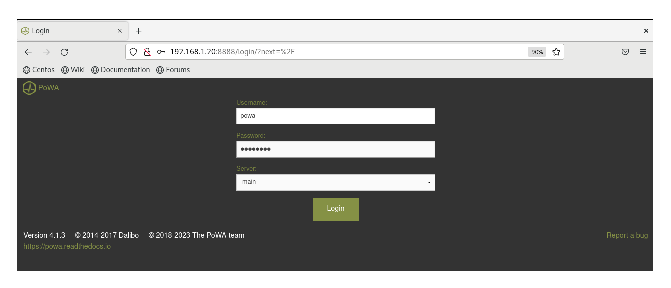
\includegraphics[angle=0, width=0.5\textwidth]{images/powa_login.eps}
\end{center}
\end{figure}

\end{frame}

%%%%%%%%%%%%%%%%%%%%%%%%%%%%%%%%%%%%%%%%%%%%%%%%%%%%%%%%%%%%%%%%%%%%%%%%%%%%%%%%

\begin{frame}{POWA - Ajout d'une base de données}

\begin{figure}
\begin{center}

\includegraphics[angle=0, width=0.5\textwidth]{images/powa_ajout_base1.eps}
\end{center}
\end{figure}

\begin{figure}
\begin{center}

\includegraphics[angle=0, width=0.5\textwidth]{images/powa_ajout_base2.eps}
\end{center}
\end{figure}


\end{frame}

%%%%%%%%%%%%%%%%%%%%%%%%%%%%%%%%%%%%%%%%%%%%%%%%%%%%%%%%%%%%%%%%%%%%%%%%%%%%%%%%

\begin{frame}{POWA - Visualisation des métriques}

\begin{figure}
\begin{center}

\includegraphics[angle=0, width=0.5\textwidth]{images/powa_metrics1.eps}
\end{center}
\end{figure}

\begin{figure}
\begin{center}
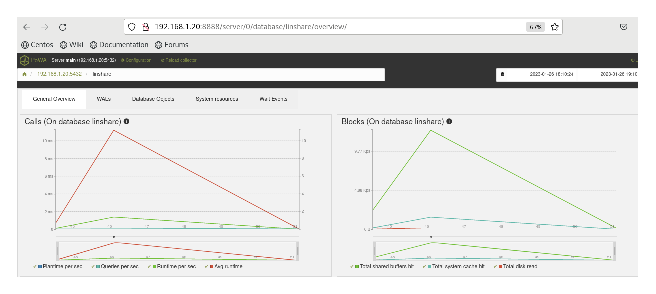
\includegraphics[angle=0, width=0.5\textwidth]{images/powa_metrics2.eps}
\end{center}
\end{figure}

\end{frame}

%%%%%%%%%%%%%%%%%%%%%%%%%%%%%%%%%%%%%%%%%%%%%%%%%%%%%%%%%%%%%%%%%%%%%%%%%%%%%%%%

\begin{frame}{pgBadger}

   \begin{itemize}
      \item pgBadger est un analyseur de logs rapide
      \item Il accepte un ou plusieurs fichiers de logs
      \item Il traite également les données fournies par l'entrée standard
      \item Il est capable de traiter un fichier de logs à distance avec un accès SSH sans mot de passe
      \item pgBadger s'appuie sur les protocoles http et ftp pour traiter les fichiers de log distants
      \item Il peut traiter les logs de pgBouncer
      \item Traitement incrémental des logs
      \item Génère des rapports au format HTML

   \end{itemize}

\begin{tiny}
\begin{toile}
\toileurl{https://pgbadger.darold.net/documentation.html}
\end{toile}
\end{tiny}

\end{frame}

%%%%%%%%%%%%%%%%%%%%%%%%%%%%%%%%%%%%%%%%%%%%%%%%%%%%%%%%%%%%%%%%%%%%%%%%%%%%%%%%

\begin{frame}{Métriques remontées par pgBadger}

   Les métriques suivantes sont remontées par pgBadger:
   \begin{itemize}
      \item Statistiques globales
      \item Requêtes les plus fréquemment en attente
      \item Requêtes ayant attendu le plus longtemps
      \item Requêtes ayant généré le plus fréquemment des fichiers temporaires
      \item Requêtes ayant généré les plus grands fichiers temporaires
      \item Requêtes les plus lentes
      \item Requêtes ayant duré le plus longtemps
      \item Requêtes les plus fréquentes
   \end{itemize}

\end{frame}

%%%%%%%%%%%%%%%%%%%%%%%%%%%%%%%%%%%%%%%%%%%%%%%%%%%%%%%%%%%%%%%%%%%%%%%%%%%%%%%%

\begin{frame}{Métriques remontées par pgBadger}

   \begin{itemize}
      \item Erreurs les plus fréquentes
      \item Histogramme du temps pris par les requêtes
      \item Histogramme du temps pris par les sessions
      \item Utilisateurs des requêtes les plus fréquentes
      \item Applications des requêtes les plus fréquentes
      \item Requêtes générant le plus d'annulation
      \item Requêtes les plus annulées
      \item Requêtes de type prepare/bind durant le plus longtemps
   \end{itemize}

\end{frame}

%%%%%%%%%%%%%%%%%%%%%%%%%%%%%%%%%%%%%%%%%%%%%%%%%%%%%%%%%%%%%%%%%%%%%%%%%%%%%%%%

\begin{frame}[fragile]{Exercice - Installer pgBadger}

   Installer pgBadger en appliquant les commandes suivantes en tant que \textbf{root}:


\begin{tiny}
\begin{Verbatim}[commandchars=\\\{\}]
[root@localhost ~]# dnf install https://dl.fedoraproject.org/pub/epel/epel-release-latest-8.noarch.rpm https://dl.fedoraproject.org/pub/epel/epel-next-release-latest-8.noarch.rpm
[root@localhost ~]# dnf install perl-Text-CSV_XS
[root@localhost ~]# dnf install pgbadger
\end{Verbatim}
\end{tiny}

\end{frame}

%%%%%%%%%%%%%%%%%%%%%%%%%%%%%%%%%%%%%%%%%%%%%%%%%%%%%%%%%%%%%%%%%%%%%%%%%%%%%%%%

\begin{frame}[fragile]{Exercice - Paramétrage préalable de PostgreSQL}

   Vérifier que la ligne suivante est présente dans postgresql.conf:

\begin{tiny}
\begin{Verbatim}[commandchars=\\\{\}]
log_min_duration_statement = 0
\end{Verbatim}
\end{tiny}

Les lignes du journal doivent avoir un minimum d'information:

\begin{tiny}
\begin{Verbatim}[commandchars=\\\{\}]
log_line_prefix = '%t [%p]: '
log_checkpoints = on
log_connections = on
log_disconnections = on
log_lock_waits = on
log_temp_files = 0
log_autovacuum_min_duration = 0
log_error_verbosity = default
\end{Verbatim}
\end{tiny}

   \textbf{Remarques:}
\begin{itemize}
   \item Ne pas activer l'option log\_statement car son format ne peut être traité par pgBadger
   \item pgBadger est restreint aux messages de log en anglais. Il ne peut traiter des logs en langue française.
\end{itemize}

\end{frame}

%%%%%%%%%%%%%%%%%%%%%%%%%%%%%%%%%%%%%%%%%%%%%%%%%%%%%%%%%%%%%%%%%%%%%%%%%%%%%%%%

\begin{frame}[fragile]{Exercice - Utilisation de pgBadger}

Pour tester l'installation, on peut lancer la commande suivante en tant que \textbf{postgres}:

\begin{tiny}
\begin{Verbatim}[commandchars=\\\{\}]
# pgbadger --help
# pgbadger /var/lib/pgsql/15/data/log/postgresql-Wed.log -o /var/www/html/pgbadger.html
\end{Verbatim}
\end{tiny}

Ce rapport peut ensuite être visualisé avec un navigateur web.

\end{frame}

%%%%%%%%%%%%%%%%%%%%%%%%%%%%%%%%%%%%%%%%%%%%%%%%%%%%%%%%%%%%%%%%%%%%%%%%%%%%%%%%

\begin{frame}{pgAdmin4 - Présentation}

   \begin{itemize}
      \item pgAdmin4 est un outil d'administration de base de données PostgreSQL
      \item Il est multi-plateforme (Microsoft Windows, Linux, MacOS)
      \item Il a une documentation fournie et détaillée
      \item Il possède 2 modes de déploiement:
      \begin{itemize}
         \item le mode desktop
         \item le mode serveur, multi-utilisateurs avec un accès web
      \end{itemize}
      \item Il intègre un éditeur de requêtes SQL avec coloration syntaxique
      \item Les données sont affichées rapidement dans une grille interactive
      \item Le plan d'exécution de la requête est affichée de manière ergonomique

   \end{itemize}

\begin{tiny}
\begin{toile}
\toileurl{https://www.pgadmin.org/}
\end{toile}
\end{tiny}

\end{frame}

%%%%%%%%%%%%%%%%%%%%%%%%%%%%%%%%%%%%%%%%%%%%%%%%%%%%%%%%%%%%%%%%%%%%%%%%%%%%%%%%

\begin{frame}{pgAdmin4 - Présentation}

   \begin{itemize}
      \item Il a un menu dédié à la gestion efficace des ACLs
      \item Débugger intégré du langage pl-pgsql
      \item Outil de diff des schémas
      \item Editeur de graphe ERD (Entity Relation Diagram) pour la conception et la documentation
      \item Outils de maintenance
      \begin{itemize}
         \item Gestion de l'autovacuum
         \item Tableau de bord de supervision
         \item Sauvegarde, restauration, vacuum et analyze à la demande
         \item Déploiement de job en SQL/shell/batch grâce un agent de programmation
      \end{itemize}
      \item Un grand nombre de jeu de caractères supportés
      \item Gestion des objets PostgreSQL (table, types, vues matérialisées, \ldots)

   \end{itemize}

\end{frame}

%%%%%%%%%%%%%%%%%%%%%%%%%%%%%%%%%%%%%%%%%%%%%%%%%%%%%%%%%%%%%%%%%%%%%%%%%%%%%%%%

\begin{frame}{Echantillon d'objets gérés par pgAdmin4}

   \begin{itemize}
      \item Contraintes d'exclusion
      \item Extensions
      \item Recherche pleine de texte - Full Text Search (FTS)
      \item Enveloppeurs de données externes - Foreign Data Wrappers
      \item Politiques de sécurité de lignes (RLS)

   \end{itemize}

\end{frame}

%%%%%%%%%%%%%%%%%%%%%%%%%%%%%%%%%%%%%%%%%%%%%%%%%%%%%%%%%%%%%%%%%%%%%%%%%%%%%%%%

\begin{frame}[fragile]{Exercice - Installation de pgAdmin4}

   \begin{itemize}
      \item Le lien ci-dessous décrit le déploiement web d'un serveur pgAdmin4

\begin{tiny}
\begin{Verbatim}[commandchars=\\\{\}]
[linagora@localhost ~]$ sudo -i
[root@localhost ~]# rpm --import https://www.pgadmin.org/static/packages_pgadmin_org.pub
[root@localhost ~]# rpm -i https://ftp.postgresql.org/pub/pgadmin/pgadmin4/yum/pgadmin4-redhat-repo-2-1.noarch.rpm
[root@localhost ~]# dnf install -y policycoreutils-python-utils
\end{Verbatim}
\end{tiny}

   \end{itemize}

\begin{tiny}
\begin{toile}
\toileurl{https://www.howtoforge.com/how-to-install-pgadmin-4-on-rocky-linux/}
\end{toile}
\end{tiny}

\end{frame}

%%%%%%%%%%%%%%%%%%%%%%%%%%%%%%%%%%%%%%%%%%%%%%%%%%%%%%%%%%%%%%%%%%%%%%%%%%%%%%%%

\begin{frame}[fragile]{Exercice - Activation du mode web}

   \begin{itemize}

\begin{tiny}
\begin{Verbatim}[commandchars=\\\{\}]
[root@localhost ~]# /usr/pgadmin4/bin/setup-web.sh
Setting up pgAdmin 4 in web mode on a Redhat based platform...
...
Email address: selbaz@linagora.com
Password: 
Retype password:
You can now start using pgAdmin 4 in web mode at http://127.0.0.1/pgadmin4
\end{Verbatim}
\end{tiny}

Pour accéder au serveur web depuis le PC, merci de créer le tunnel SSH équivalent avec PuttY:
\begin{tiny}
\begin{Verbatim}[commandchars=\\\{\}]
# ssh -L 9090:10.10.10.28:80 hqpg-sandbox
\end{Verbatim}
\end{tiny}

Puis entrer l'URL:
\begin{tiny}
\begin{Verbatim}[commandchars=\\\{\}]
http://127.0.0.1:9090/pgadmin4
\end{Verbatim}
\end{tiny}

\end{itemize}

\end{frame}

%%%%%%%%%%%%%%%%%%%%%%%%%%%%%%%%%%%%%%%%%%%%%%%%%%%%%%%%%%%%%%%%%%%%%%%%%%%%%%%%

\begin{frame}[fragile]{Exercice - pgadmin4 screenshots}

\begin{figure}
\begin{center}
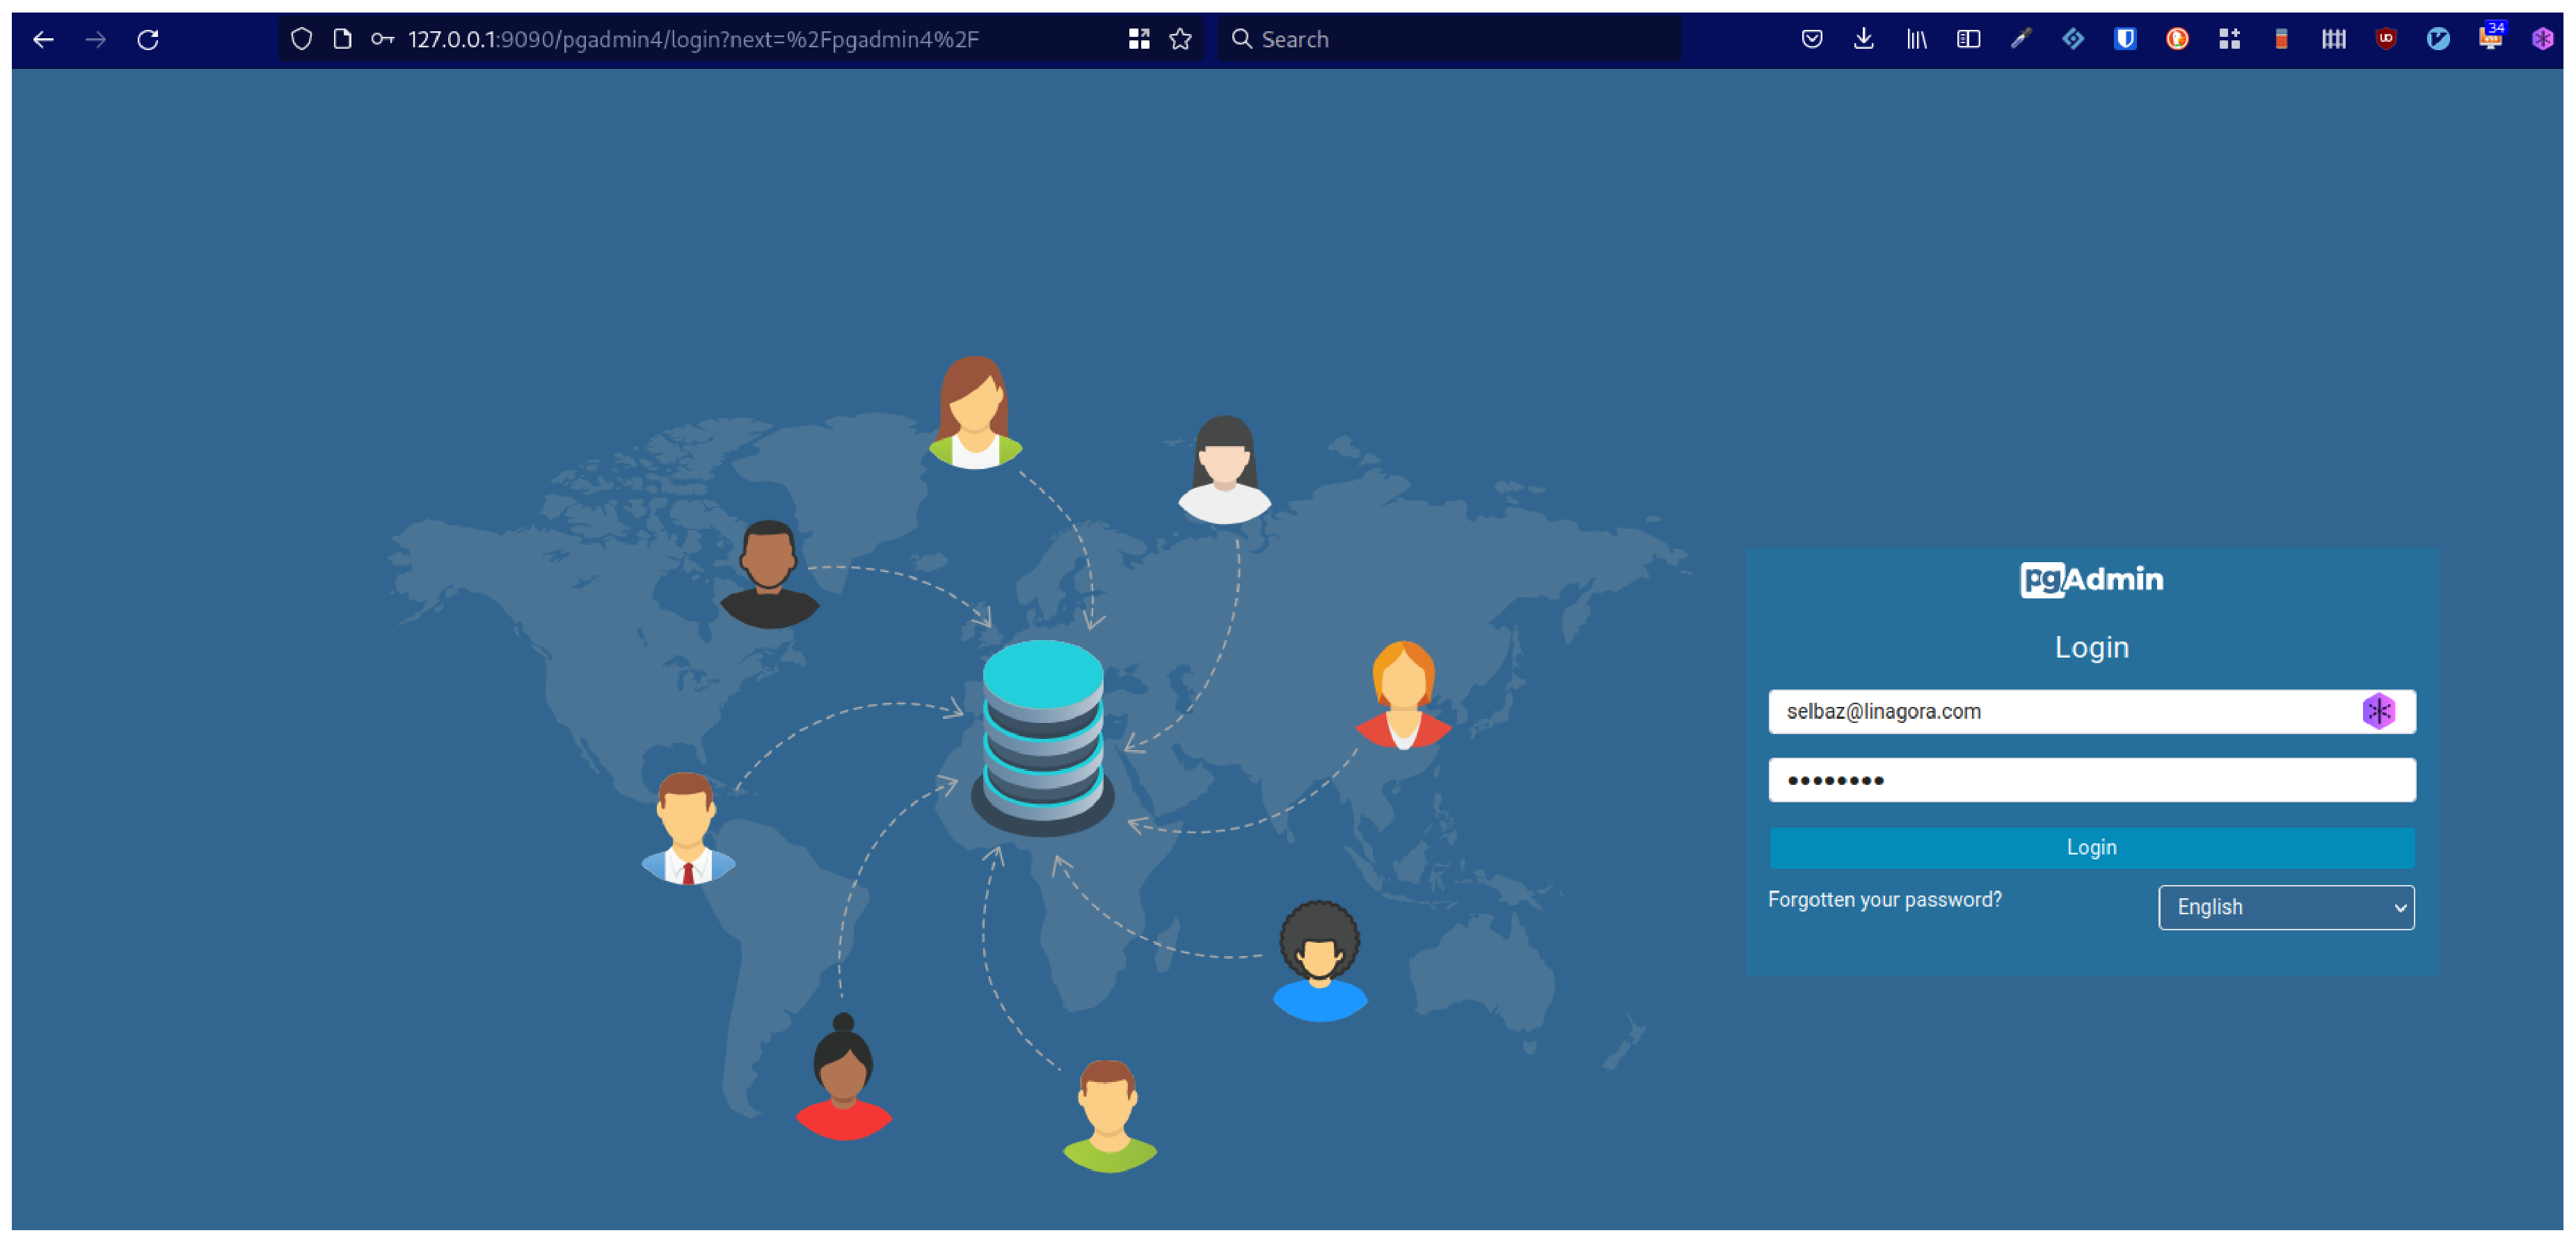
\includegraphics[angle=0, width=0.5\textwidth]{images/pgadmin4_login.eps}
\end{center}
\end{figure}

\begin{figure}
\begin{center}
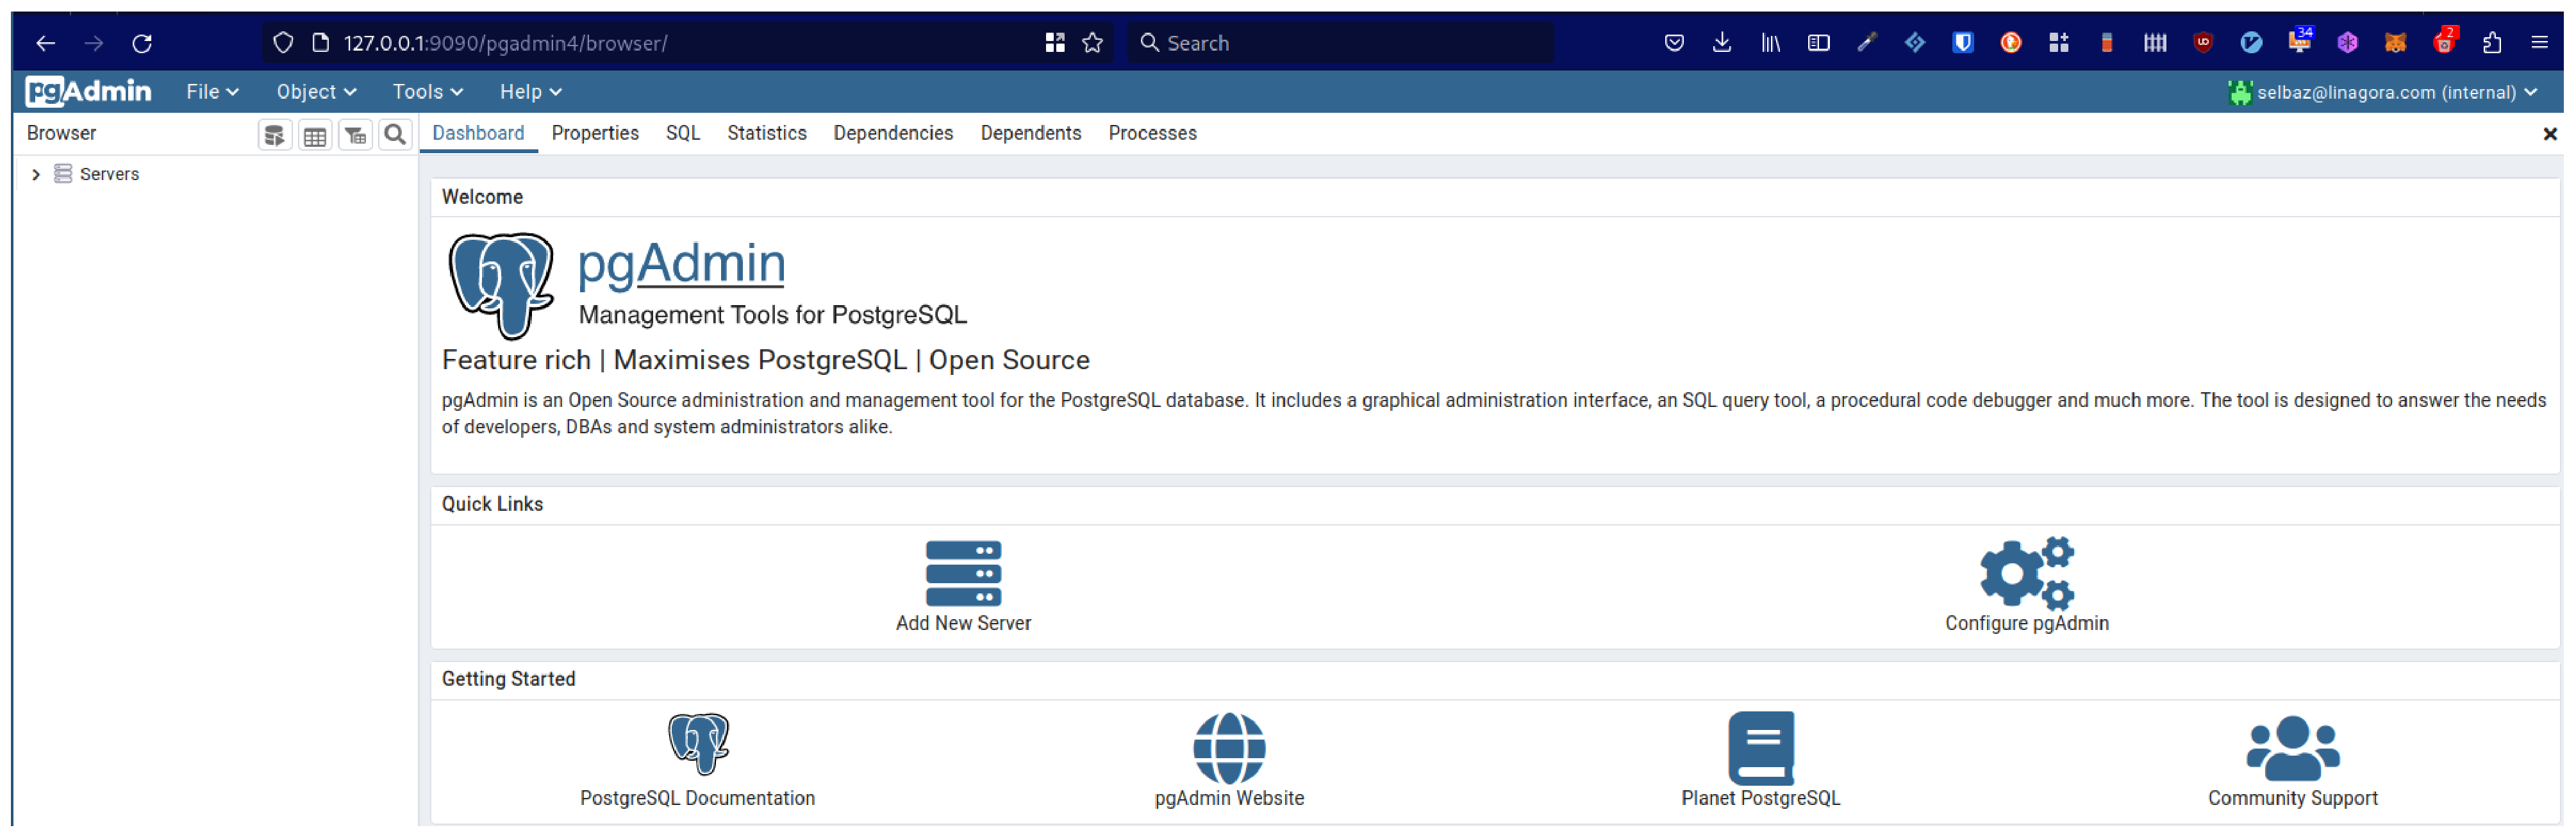
\includegraphics[angle=0, width=0.5\textwidth]{images/pgadmin4_home.eps}
\end{center}
\end{figure}

\end{frame}

%%%%%%%%%%%%%%%%%%%%%%%%%%%%%%%%%%%%%%%%%%%%%%%%%%%%%%%%%%%%%%%%%%%%%%%%%%%%%%%%

\begin{frame}[fragile]{Exercice - pgadmin4 screenshots}

\begin{figure}
\begin{center}
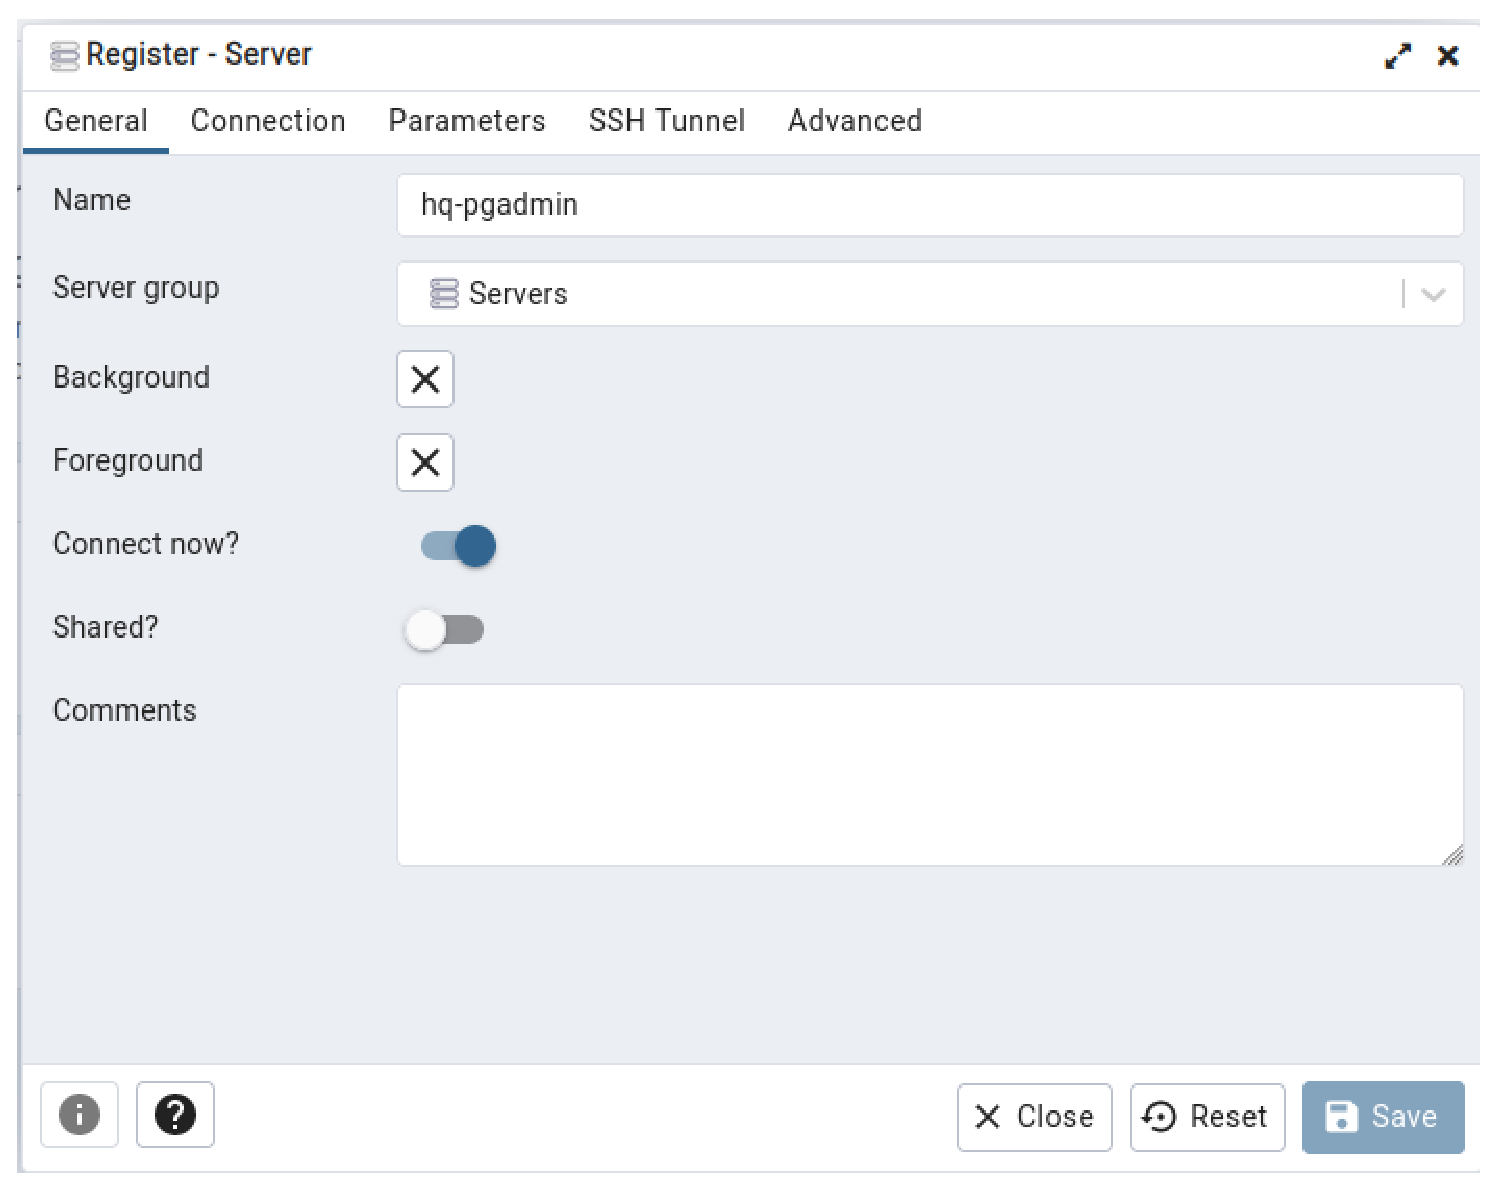
\includegraphics[angle=0, width=0.5\textwidth]{images/pgadmin4_connexiondb.eps}
\end{center}
\end{figure}

\end{frame}

%%%%%%%%%%%%%%%%%%%%%%%%%%%%%%%%%%%%%%%%%%%%%%%%%%%%%%%%%%%%%%%%%%%%%%%%%%%%%%%%

\section{Point In Time Recovery}

%%%%%%%%%%%%%%%%%%%%%%%%%%%%%%%%%%%%%%%%%%%%%%%%%%%%%%%%%%%%%%%%%%%%%%%%%%%%%%%%

\begin{frame}{Cycle des données dans PostgreSQL}

\begin{figure}
\begin{center}
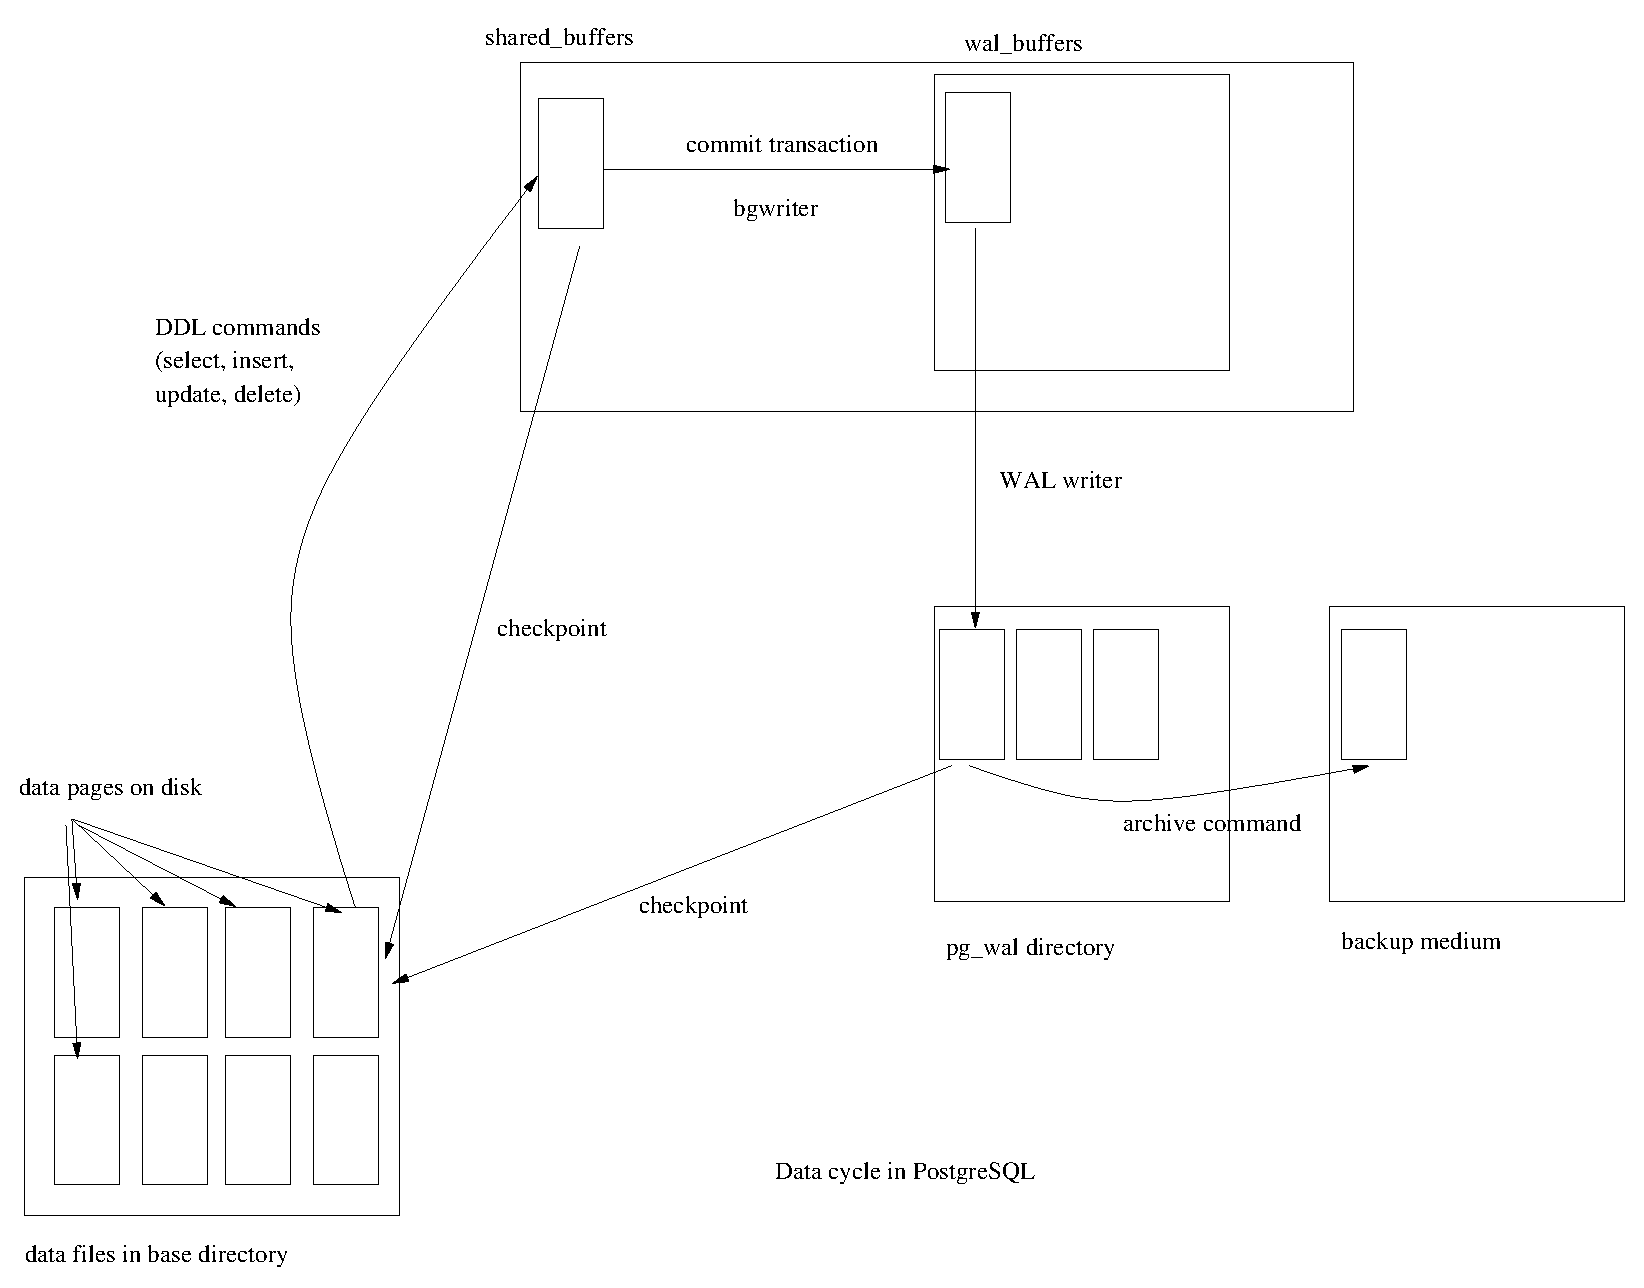
\includegraphics[angle=0, width=0.5\textwidth]{images/internals.eps}
\end{center}
\end{figure}

\begin{toile}
\toileurl{https://www.postgresql.org/docs/15/wal-configuration.html}
\end{toile}

\end{frame}

%%%%%%%%%%%%%%%%%%%%%%%%%%%%%%%%%%%%%%%%%%%%%%%%%%%%%%%%%%%%%%%%%%%%%%%%%%%%%%%%

\begin{frame}{Multiversion Concurrency Control - MVCC}

   \begin{itemize}
      \item PostgreSQL fournit un grand nombre d'outils pour gérer l'accès concurrentiel aux données
      \item De manière interne, la ochérence des données est mise en place en utilisant un modèle multi-versions (MVCC)
      \item Cela signifie que chaque requête SQL a la vision d'un instantané des données (snapshot)
      \item Cet instantané correspond à une version de la base de données il y a quelques instants, quelques soient les modifications actuellement réalisées sur les données
      \item Cela empêche les requêtes de voir des données incohérentes modifiées par des requêtes parallèle
      \item Cette méthode fournit l'isolation transactionnelle pour chaque session de la base des données
   \end{itemize}

\begin{toile}
\toileurl{https://www.postgresql.org/docs/15/mvcc-intro.html}
\end{toile}

\end{frame}

%%%%%%%%%%%%%%%%%%%%%%%%%%%%%%%%%%%%%%%%%%%%%%%%%%%%%%%%%%%%%%%%%%%%%%%%%%%%%%%%

\begin{frame}{Multiversion Concurrency Control - MVCC}

   \begin{itemize}
      \item Le MVCC en évitant les méthodes de verrouillage des bases de données classiques minimise la contention et favorise la performance dans un environnement multi-utilisateurs
      \item En cas de nécessité de verrouillage, il existe différents type de verrous:
      \begin{itemize}
         \item le verrouillage en lecture
         \item le verrouillage en écriture
         \item ces 2 types de verrous ne se gênent pas mutuellement: un verrou en lecture n'empêche pas l'écriture et vice-versa 
      \end{itemize}
   \end{itemize}

\end{frame}

%%%%%%%%%%%%%%%%%%%%%%%%%%%%%%%%%%%%%%%%%%%%%%%%%%%%%%%%%%%%%%%%%%%%%%%%%%%%%%%%

\begin{frame}[fragile]{Mise en place de la génération des WAL}

\begin{itemize}

   \item Pour activer la génération des WAL, merci de modifier les paramètres suivants dans \textit{postgresql.conf}

\begin{intercom}
wal\_level = replica # or higher
archive\_mode = on
[...]
\end{intercom}

\end{itemize}

\begin{toile}
\toileurl{https://www.postgresql.org/docs/15/continuous-archiving.html}
\end{toile}

\end{frame}

%%%%%%%%%%%%%%%%%%%%%%%%%%%%%%%%%%%%%%%%%%%%%%%%%%%%%%%%%%%%%%%%%%%%%%%%%%%%%%%%

\begin{frame}[fragile]{\commande{archive\_command} et \commande{archive\_library}}

\begin{itemize}

   \item La copie des WAL vers le système de sauvegarde se paramètre depuis les 2 valeurs suivantes:

   \begin{itemize}
      \item \textbf{archive\_command}: Commandes shell d'archivage des WAL
      \item \textbf{archive\_library}: Binaire d'archivage des WAL
   \end{itemize}

   \item Chacune des 2 valeurs s'utilise au choix. Elles ne peuvent utilisées en même temps.
   \item Pour les exercices, le paramètre \textbf{archive\_command} sera utilisé.

\begin{tiny}
\begin{Verbatim}[commandchars=\\\{\}]
archive\_command = 'test ! -f /mnt/server/archivedir/\%f && cp \%p /mnt/server/archivedir/\%f' # Unix
   [...]
\end{Verbatim}
\end{tiny}

\end{itemize}

\end{frame}

%%%%%%%%%%%%%%%%%%%%%%%%%%%%%%%%%%%%%%%%%%%%%%%%%%%%%%%%%%%%%%%%%%%%%%%%%%%%%%%%

\begin{frame}[fragile]{Fonctionnement de l'archivage des WAL}

\begin{itemize}

   \item La commande d'archivage des WALs est lancée par le même utilisateur du process \textit{postmaster}
   \item Elle est censée renvoyer un code différent de 0 en cas d'erreur
   \item Il est important de vérifier que le WAL n'existe pas dans le répertoire cible sous peine de l'écraser
   \item En cas d'erreur d'archivage, PostgreSQL retente autant de fois que nécessaire
   \item Tant que le fichier WAL n'est pas archivé, celui-ci n'est pas supprimé du répertoire pg\_wal, ce qui peut amener à une saturation du système de fichiers
   \item En cas de saturation du répertoire pg\_wal, le serveur s'arrête avec une erreur de type PANIC. Il pourra redémarrer une fois qu'il aura de l'espace disque disponible

\end{itemize}

\end{frame}

%%%%%%%%%%%%%%%%%%%%%%%%%%%%%%%%%%%%%%%%%%%%%%%%%%%%%%%%%%%%%%%%%%%%%%%%%%%%%%%%

\begin{frame}[fragile]{Caractéristiques des WAL}

\begin{itemize}

   \item Le nom des fichiers WAL inclut jusqu'à 64 caractères
   \item Il est composé de lettres ASCII, de chiffres et de points
   \item Il est important de garder le nom de l'archive WAL
   \item La sauvegarde des WALs ne permet pas de restaurer \textit{postgresql.conf}, \textit{pg\_hba.conf} ou \textit{pg\_ident.conf}
   \item Il est important de sauvegarder ces 3 fichiers indépendamment
   \item Ces fichiers peuvent être stockés dans un répertoire paramétrable

\end{itemize}

\end{frame}

%%%%%%%%%%%%%%%%%%%%%%%%%%%%%%%%%%%%%%%%%%%%%%%%%%%%%%%%%%%%%%%%%%%%%%%%%%%%%%%%

\begin{frame}[fragile]{Timelines (lignes de temps)}

\begin{itemize}

   \item Après chaque opération de recovery, PostgreSQL créée une nouvelle ligne de temps (timeline)
   \item Au passage, le serveur crée un fichier "timeline history" qui lui indique la série de WAL générés après le recovery
   \item Les WALs créés après l'opération de recovery appartiennent à cette nouvelle ligne de temps
   \item Par défaut, l'opération de recovery rétablit la timeline la plus récente
   \item Il est possible de rétablir une timeline donnée dans le passé


\end{itemize}

\begin{toile}
\toileurl{https://www.postgresql.org/docs/15/continuous-archiving.html}
\end{toile}

\end{frame}


%%%%%%%%%%%%%%%%%%%%%%%%%%%%%%%%%%%%%%%%%%%%%%%%%%%%%%%%%%%%%%%%%%%%%%%%%%%%%%%%

\begin{frame}[fragile]{Format du nom du WAL}

   Dans le répertoire /pg\_wal, on peut voir le WAL suivant:

\begin{itemize}

   \item \textbf{00000001}000000000000001B
   \item La timeline est représentée par les 8 premiers chiffres du nom du WAL

\end{itemize}

\begin{toile}
\toileurl{https://www.postgresql.org/docs/15/continuous-archiving.html}
\end{toile}

\end{frame}


%%%%%%%%%%%%%%%%%%%%%%%%%%%%%%%%%%%%%%%%%%%%%%%%%%%%%%%%%%%%%%%%%%%%%%%%%%%%%%%%

\begin{frame}[fragile]{La commande \commande{pg\_basebackup}}

\begin{itemize}

\item La commande \commande{pg\_basebackup} sauvegarde un cluster PostgreSQL
\item Elle ne s'applique pas sur une base de données en particulier
\item L'utilisateur lançant cette commande doit posséder le droit \textbf{REPLICATION} ou être un super-utilisateur
\item La commande peut être lancée sur un serveur standby
\item La table \textit{pg\_stat\_progress\_basebackup} donne une idée de la progression de la commande

\end{itemize}

\begin{toile}
\toileurl{https://www.postgresql.org/docs/15/app-pgbasebackup.html}
\toileurl{https://www.postgresql.org/docs/15/progress-reporting.html\#BASEBACKUP-PROGRESS-REPORTING}
\end{toile}

\end{frame}

%%%%%%%%%%%%%%%%%%%%%%%%%%%%%%%%%%%%%%%%%%%%%%%%%%%%%%%%%%%%%%%%%%%%%%%%%%%%%%%%

\begin{frame}{Options de la commande \commande{pg\_basebackup}}

   Les options qui semblent les plus intéressantes sont:

\begin{itemize}

   \item \option{-F \textit{format}}
   \item \textit{format} a les valeurs suivantes:
   \begin{itemize}
      \item  \textit{p} ou \textit{plain}. Format par défaut. 
      \item  \textit{t} ou \textit{tar}. Génération d'une archive du répertoire des données \textit{base.tar}
   \end{itemize}

\end{itemize}

\begin{toile}
\toileurl{https://www.postgresql.org/docs/15/app-pgbasebackup.html}
\end{toile}

\end{frame}

%%%%%%%%%%%%%%%%%%%%%%%%%%%%%%%%%%%%%%%%%%%%%%%%%%%%%%%%%%%%%%%%%%%%%%%%%%%%%%%%

\begin{frame}{Options de la commande \commande{pg\_basebackup}}

\begin{itemize}
   \item \option{-R} or \option{{-}{-}write-recovery-conf}
   \begin{itemize}
      \item la commande génère automatiquement le fichier \textbf{standby.signal}
   \end{itemize}
   \item \option{-T \textit{olddir}=\textit{newdir}} ou \option{{-}{-}tablespace-mapping=\textit{olddir}=\textit{newdir}}
   \begin{itemize}
      \item cette option permet de mapper les répertoires du serveur liés aux tablespaces à d'autres répertoires locaux. Option valide uniquement si le format \textbf{plain} est utilisé. 
   \end{itemize}
   \item \option{-X \textit{method}} ou \option{{-}{-}wal-method=\textit{method}}
   \begin{itemize}
   \item \textit{method} a les valeurs suivantes:
      \begin{itemize}
         \item  \textit{n} ou \textit{none}. Le backup n'inclut pas les WAL.
         \item  \textit{f} ou \textit{fetch}. Les WAL générés durant le backup sont récupérés une fois le backup généré. Dans le cas de l'utilisation de cette option, le paramètre \option{wal\_keep\_size} nécessite d'être ajusté correctement afin que le serveur puisse garder l'ensemble des WAL (et ne supprime ni n'en recycle durant le backup).
         \item  \textit{s} ou \textit{stream}. Mode par défaut. Une $2^{\grave{e}me}$ connexion est établie vers le serveur pour streamer les WAL générés durant le backup.
      \end{itemize}
   \end{itemize}
\end{itemize}

\end{frame}

%%%%%%%%%%%%%%%%%%%%%%%%%%%%%%%%%%%%%%%%%%%%%%%%%%%%%%%%%%%%%%%%%%%%%%%%%%%%%%%%

\begin{frame}{Options de la commande \commande{pg\_basebackup}}

\begin{itemize}
   \item \option{{-}{-}no-estimate-size}
   \begin{itemize}
      \item le serveur n'estime plus la taille du backup avant de débuter le process. Cela permet de raccourcir la durée de la génération du backup.
   \end{itemize}

\item{\textbf{Environment}}
   \begin{itemize}
      \item Cet utilitaire, tout comme la majorité des utilitaires PostgreSQL, utilisent les mêmes variables d'environnement que ceux de la libpq.
      \item La variable d'environment PG\_COLOR indique si la couleur est utilisée dans les messages de diagnostique. Les valeurs possibles sont \textsl{always}, \textsl{auto} et \textsl{never}.
   \end{itemize}
\end{itemize}

\end{frame}

%%%%%%%%%%%%%%%%%%%%%%%%%%%%%%%%%%%%%%%%%%%%%%%%%%%%%%%%%%%%%%%%%%%%%%%%%%%%%%%%

\begin{frame}{Checkpoints}
   \label{checkpoint}

\begin{itemize}
   \item A chaque checkpoint, l'ensemble des pages chargées et modifiées (\textsf{dirty pages}) dans les \textsf{shared\_buffers} sont flushées en disque.
   \item Les données présentes dans les WAL sont également écrites en disque.
   \item En cas de rejeu des WAL (\textbf{REDO}), le serveur part de la dernière transaction liée au checkpoint pour rejouer les WALs.
   \item Cette opération engendre une forte activité I/O
   \item La fréquence des checkpoint est liée à 2 paramètres:
   \begin{itemize}
      \item \textbf{checkpoint\_timeout}
      \item \textbf{max\_wal\_size}
   \end{itemize}
\end{itemize}

\begin{toile}
\toileurl{https://www.postgresql.org/docs/current/wal-configuration.html}
\end{toile}

\end{frame}

%%%%%%%%%%%%%%%%%%%%%%%%%%%%%%%%%%%%%%%%%%%%%%%%%%%%%%%%%%%%%%%%%%%%%%%%%%%%%%%%

\begin{frame}{\textbf{checkpoint\_timeout} et \textbf{max\_wal\_size}}

   \textbf{checkpoint\_timeout}
\begin{itemize}
   \item Intervalle en secondes entre 2 checkpoints automatiques
\end{itemize}

   \textbf{max\_wal\_size}
\begin{itemize}
   \item Taille disque maximale occupée par les WAL. Lorsque cette taille est atteinte, l'opération de checkpoint est déclenchée ainsi que \textsf{archive\_command}.
\end{itemize}

   \textbf{min\_wal\_size}
\begin{itemize}
   \item Taille disque minimale occupée par les WAL. Lorsque ce seuil est atteint, les WAL ne sont plus supprimés mais recyclés (renommés).
\end{itemize}

\begin{toile}
\toileurl{https://www.postgresql.org/docs/current/runtime-config-wal.html\#GUC-CHECKPOINT-TIMEOUT}
\toileurl{https://www.postgresql.org/docs/current/runtime-config-wal.html\#GUC-MAX-WAL-SIZE}
\end{toile}

\end{frame}

%%%%%%%%%%%%%%%%%%%%%%%%%%%%%%%%%%%%%%%%%%%%%%%%%%%%%%%%%%%%%%%%%%%%%%%%%%%%%%%%

\begin{frame}[fragile]{La commande \commande{pg\_verifybackup}}

\begin{itemize}

   \item La commande \commande{pg\_verifybackup} vérifie l'intégrité d'une sauvegarde générée par la commande \commande{pg\_basebackup}
   \item Elle s'applique sur un backup généré au format plain. Dans le cas de la vérification d'une archive tar, il est nécessaire de désarchiver auparavant.

\end{itemize}

\begin{toile}
\toileurl{https://www.postgresql.org/docs/15/app-pgverifybackup.html}
\end{toile}

\end{frame}

%%%%%%%%%%%%%%%%%%%%%%%%%%%%%%%%%%%%%%%%%%%%%%%%%%%%%%%%%%%%%%%%%%%%%%%%%%%%%%%%

\begin{frame}[fragile]{La commande \commande{pg\_amcheck}}

\begin{itemize}

   \item La commande \commande{pg\_amcheck} vérifie l'intégrité d'une base de données.
   \item Fait appel à l'utilitaire \textsf{amcheck}
   \item S'applique aux tables ordinaires, celles de type TOAST, les vues matérialisées, les séquences, les indexes btree.
   \item Possède des options de filtrages de base, de schéma et de table

\end{itemize}

\begin{toile}
\toileurl{https://www.postgresql.org/docs/current/app-pgamcheck.html}
\toileurl{https://www.postgresql.org/docs/current/amcheck.html}
\end{toile}

\end{frame}

%%%%%%%%%%%%%%%%%%%%%%%%%%%%%%%%%%%%%%%%%%%%%%%%%%%%%%%%%%%%%%%%%%%%%%%%%%%%%%%%

\begin{frame}[fragile]{Principales options de la commande \commande{pg\_amcheck}}

   Les principales options de cette commande sont:

\begin{itemize}

   \item \option{{-}{-}no-dependent-indexes} exclut de la vérification les indexes associés à la table
   \item \option{{-}{-}no-dependent-toast} exclut de la vérification les tables TOAST associées à la table
   \item Options applicables aux indexes

   \begin{itemize}
      \item \option{{-}{-}heapallindexed} crée un nouvel index temporaire en mémoire pour vérifier que l'index actuellement stocké est valide. Cette option utilise de la RAM limitée par le paramètre \option{maintenance\_work\_mem}
   \end{itemize}
\end{itemize}

\end{frame}

%%%%%%%%%%%%%%%%%%%%%%%%%%%%%%%%%%%%%%%%%%%%%%%%%%%%%%%%%%%%%%%%%%%%%%%%%%%%%%%%

\begin{frame}{Options de la commande \commande{pg\_amcheck}}

\begin{itemize}
   \item \option{{-}{-}parent-check} vérifie les indexes de la table parent\footnote{https://www.postgresql.org/docs/current/ddl-inherit.html}
\end{itemize}

\end{frame}

%%%%%%%%%%%%%%%%%%%%%%%%%%%%%%%%%%%%%%%%%%%%%%%%%%%%%%%%%%%%%%%%%%%%%%%%%%%%%%%%

\section{Exercice}

%%%%%%%%%%%%%%%%%%%%%%%%%%%%%%%%%%%%%%%%%%%%%%%%%%%%%%%%%%%%%%%%%%%%%%%%%%%%%%%%

\begin{frame}{Réalisation d'un backup full de la base de données}

La procédure de déroulement du PITR s'appuie sur:
\begin{itemize}
   \item la génération d'un backup full
   \item l'archivage des WALs
\end{itemize}


Il existe 2 méthodes pour réaliser une sauvegarde full de la base données:
\begin{itemize}
   \item l'outil \textsf{pg\_basebackup}
   \item l'API bas niveau avec des appels aux fonctions PostgreSQL
\end{itemize}

La méthode étudiée pendant les exercices est l'outil \textsf{pg\_basebackup}.

\end{frame}

%%%%%%%%%%%%%%%%%%%%%%%%%%%%%%%%%%%%%%%%%%%%%%%%%%%%%%%%%%%%%%%%%%%%%%%%%%%%%%%%

\begin{frame}[fragile]\frametitle{Mise en place de l'archivage des WALs}

\begin{itemize}
   \item Vérifier que PostgreSQL est déployé sur les serveurs \textsf{hqpg-0x} et \textsf{hqpg-0x-repl}
   \item Mettre en place la copie des WAL vers le répertoire \path{/opt/wal_backup} avec le niveau \textbf{replica}
   \item La commande \textsf{archive\_command} s'appuie sur rsync pour transférer les WALs depuis le primaire. Pour éviter d'avoir à indiquer le mot de l'utilisateur postgres, réaliser la génération et l'échange mutuel de clefs SSH sur les 2 serveurs comme décrit en page ~\ref{sec:ssh-keys}
   \item Paramétrer la commande \textsf{archive\_command} dans postgresql.conf
   \begin{tiny}
      \item \commande{archive\_command = 'rsync \%p hqpg-0x-repl:/opt/wal\_backup/\%f'}
   \end{tiny}

\end{itemize}

\end{frame}

%%%%%%%%%%%%%%%%%%%%%%%%%%%%%%%%%%%%%%%%%%%%%%%%%%%%%%%%%%%%%%%%%%%%%%%%%%%%%%%%

\begin{frame}[fragile]\frametitle{Résumé du paramétrage de la sauvegarde des WALs}

Sur le serveur principal, les lignes suivantes sont inclues dans postgresql.conf:
\begin{tiny}
\begin{verbatim}
# Add settings for extensions here
listen_addresses = '*'
wal_level = replica
archive_mode = on
archive_command = 'rsync %p 10.10.10.29:/opt/archivedir/%f'
\end{verbatim}
\end{tiny}

\begin{itemize}
   \item Sur le serveur de sauvegarde, créer le répertoire \path{/opt/wal_backup/} de sauvegarde des WALs avec l'utilisateur postgres
\end{itemize}

\end{frame}

%%%%%%%%%%%%%%%%%%%%%%%%%%%%%%%%%%%%%%%%%%%%%%%%%%%%%%%%%%%%%%%%%%%%%%%%%%%%%%%%

\begin{frame}[fragile]\frametitle{Remarque importante sur la procédure de PITR}

\begin{small}
   \textbf{Remarque} Le point de restauration est obligatoirement après la date de fin du base backup, c'est à dire, le temps de fin de l'appel à pg\_basebackup\_stop. Il n'est possible de restaurer des données à une date durant laquelle le backup est en cours.
Pour restaurer à une telle date, il est nécessaire de restaurer le précédent backup et de rejouer les sauvegardes WALs jusqu'à ce point.
\end{small}

\end{frame}

%%%%%%%%%%%%%%%%%%%%%%%%%%%%%%%%%%%%%%%%%%%%%%%%%%%%%%%%%%%%%%%%%%%%%%%%%%%%%%%%

\begin{frame}[fragile]\frametitle{Utilisation de \textsf{pg\_basebackup} pour sauvegarder la base de données}

Sur le serveur principal, ajouter la ligne suivante dans pg\_hba.conf:

\begin{tiny}
\begin{Verbatim}[commandchars=\\\{\}]
host  replication  postgres   10.10.10.0/24  trust
\end{Verbatim}
\end{tiny}

Recharger le paramétrage avec la commande suivante:

\begin{tiny}
\begin{verbatim}
postgres=# SELECT pg_reload_conf();
\end{verbatim}
\end{tiny}

\end{frame}

%%%%%%%%%%%%%%%%%%%%%%%%%%%%%%%%%%%%%%%%%%%%%%%%%%%%%%%%%%%%%%%%%%%%%%%%%%%%%%%%

\begin{frame}[fragile]\frametitle{Génération d'un backup full}

Sur le serveur de sauvegarde des WAL, appliquer les commandes suivantes:

\begin{itemize}
   \item Comme indiqué dans\footnote{https://www.postgresql.org/docs/current/app-pgbasebackup.html}, la commande \textsf{pg\_basebackup} réalise un checkpoint (p. \ref{checkpoint}) sur le serveur
   \item \commande{pg\_basebackup -h hqpg-0x -Ft -z -P -D /opt/backup/20230213}
\end{itemize}

\end{frame}

%%%%%%%%%%%%%%%%%%%%%%%%%%%%%%%%%%%%%%%%%%%%%%%%%%%%%%%%%%%%%%%%%%%%%%%%%%%%%%%%

\begin{frame}[fragile]\frametitle{Inspection de l'archive générée}

\begin{tiny}
\begin{verbatim}
[postgres@localhost 20230202_1]$ ls -lrt
total 4420
-rw------- 1 postgres postgres  181880  2 févr. 07:58 backup_manifest
-rw------- 1 postgres postgres 4321056  2 févr. 07:58 base.tar.gz
-rw------- 1 postgres postgres   17075  2 févr. 07:58 pg_wal.tar.gz
\end{verbatim}
\end{tiny}

\begin{itemize}
   \item backup\_manifest inclut le listing avec les checkum de l'archive base.tar.gz
   \item pg\_wal.tar.gz inclut les WAL générés durant l'opération du pg\_basebackup
\end{itemize}

\end{frame}

%%%%%%%%%%%%%%%%%%%%%%%%%%%%%%%%%%%%%%%%%%%%%%%%%%%%%%%%%%%%%%%%%%%%%%%%%%%%%%%%

\begin{frame}[fragile]\frametitle{Création du jeu de données}

Sur le serveur principal, lancer les commandes suivantes:

\begin{tiny}
\begin{verbatim}
su - postgres
creatuser hq -d
createdb hqdb -O hq
psql hqdb
-- 02/02/2023 16h27
create table test_pitr1 (col1 text);
create table test_pitr2 (col1 text);
-- quelques minutes plus tard
-- 16h30
create table test_pitr3 (col1 text);
\end{verbatim}
\end{tiny}

\begin{toile}
\toileurl{https://www.postgresql.org/docs/current/app-createuser.html}
\toileurl{https://www.postgresql.org/docs/current/app-createdb.html}
\end{toile}


\end{frame}

%%%%%%%%%%%%%%%%%%%%%%%%%%%%%%%%%%%%%%%%%%%%%%%%%%%%%%%%%%%%%%%%%%%%%%%%%%%%%%%%

\begin{frame}[fragile]\frametitle{Restauration de la base de données à une date donnée}

Sur le serveur PostgreSQL principal,

\begin{tiny}
\begin{verbatim}
[root@localhost 15]# systemctl stop postgresql-15.service
[root@localhost 15]# su - postgres
Dernière connexion : samedi  4 février 2023 à 20:01:48 EST sur pts/0
[postgres@localhost ~]$ cd 15
# mv data data.20230213
# scp 10.10.10.29:/opt/backup/20230205_1/* .
# rm -rf data && mkdir data && chmod 0700 data
# tar xvzf ../base.tar.gz 
# cd pg_wal/
# tar xvzf ../../pg_wal.tar.gz 
#  cd ..
#  touch recovery.signal
\end{verbatim}
\end{tiny}

\begin{toile}
\toileurl{https://www.postgresql.org/docs/15/runtime-config-wal.html\#RUNTIME-CONFIG-WAL-RECOVERY-TARGET}
\end{toile}

\end{frame}

%%%%%%%%%%%%%%%%%%%%%%%%%%%%%%%%%%%%%%%%%%%%%%%%%%%%%%%%%%%%%%%%%%%%%%%%%%%%%%%%

\begin{frame}[fragile]\frametitle{Restauration de la base de données à une date donnée}

Ajouter les lignes suivantes dans postgresql.conf

\begin{tiny}
\begin{verbatim}
restore_command = 'rsync 10.10.10.29:/opt/archivedir/%f %p'
recovery_target_time = '2023-02-05 02:20:00+01'
\end{verbatim}
\end{tiny}

Démarrer le serveur avec la commande.

\end{frame}

%%%%%%%%%%%%%%%%%%%%%%%%%%%%%%%%%%%%%%%%%%%%%%%%%%%%%%%%%%%%%%%%%%%%%%%%%%%%%%%%

\begin{frame}[fragile]\frametitle{Logs de la restauration}

\begin{tiny}
\begin{Verbatim}[commandchars=\\\{\}]
rsync: link_stat "/opt/archivedir/00000002.history" failed: No such file or directory (2)
rsync error: some files/attrs were not transferred (see previous errors) (code 23) at main.c(1670) [Receiver=3.1.3]
2023-02-04 20:28:02.203 EST [22385] LOG:  début de la restauration de l'archive à \userinput{2023-02-04 20:20:00-05}
2023-02-04 20:28:03.278 EST [22385] LOG:  la ré-exécution commence à 0/1C000028
2023-02-04 20:28:03.648 EST [22385] LOG:  restauration du journal de transactions « 00000001000000000000001D » à partir de l'archive
2023-02-04 20:28:05.011 EST [22385] LOG:  état de restauration cohérent atteint à 0/1C000100
2023-02-04 20:28:05.011 EST [22381] LOG:  le système de bases de données est prêt pour accepter les connexions en lecture seule
rsync: link_stat "/opt/archivedir/00000001000000000000001F" failed: No such file or directory (2)
2023-02-04 20:28:05.172 EST [22385] LOG:  arrêt de la restauration avant validation de la transaction 740, 2023-02-04 20:21:11.941687-05
2023-02-04 20:28:05.172 EST [22385] LOG:  pause à la fin de la restauration
2023-02-04 20:28:05.172 EST [22385] \userinput{ASTUCE :  Exécuter pg_wal_replay_resume() pour promouvoir.}
2023-02-04 20:33:01.702 EST [22383] LOG:  début du restartpoint : time
2023-02-04 20:33:05.828 EST [22383] LOG:  restartpoint terminé : a écrit 26 tampons (0.2%); 0 fichiers WAL ajoutés, 2 supprimés, 0 recyclés ; écriture=3.090 s, synchronisation=0.610 s, total=4.127 s; fichiers synchronisés=18, plus long=0.609 s, moyenne=0.034 s; distance=32768 kB, estimation=32768 kB
2023-02-04 20:33:05.829 EST [22383] LOG:  la ré-exécution en restauration commence à 0/1E000028
\end{Verbatim}
\end{tiny}

\end{frame}

%%%%%%%%%%%%%%%%%%%%%%%%%%%%%%%%%%%%%%%%%%%%%%%%%%%%%%%%%%%%%%%%%%%%%%%%%%%%%%%%

\begin{frame}[fragile]\frametitle{Basculement de la base de données en mode écriture}

\begin{tiny}
\begin{verbatim}
hqdb=# create table test_pitr_20230206144000 (col1 text);
ERREUR:  ne peut pas exécuter CREATE TABLE dans une transaction en lecture seule
hqdb=# quit
[postgres@localhost pg_wal]$ psql
psql (15.1)
Saisissez « help » pour l'aide.

postgres=# select pg_wal_replay_resume();
 pg_wal_replay_resume 
----------------------
 
(1 ligne)

postgres=# create table test_pitr_20230206144000 (col1 text);
CREATE TABLE
\end{verbatim}
\end{tiny}

\end{frame}

%%%%%%%%%%%%%%%%%%%%%%%%%%%%%%%%%%%%%%%%%%%%%%%%%%%%%%%%%%%%%%%%%%%%%%%%%%%%%%%%

\begin{frame}[fragile]\frametitle{Apparition d'une nouvelle ligne de temps}

\begin{tiny}
\begin{Verbatim}[commandchars=\\\{\}]
[postgres@localhost pg_wal]$ ls -lrt
total 32772
-rw------- 1 postgres postgres 16777216  6 févr. 08:41 00000001000000000000001E
\userinput{-rw------- 1 postgres postgres       51  6 févr. 08:41 00000002.history}
drwx------ 2 postgres postgres       72  6 févr. 08:41 archive_status
\userinput{-rw------- 1 postgres postgres 16777216  6 févr. 08:46 00000002000000000000001E}
\end{Verbatim}
\end{tiny}

\end{frame}

%%%%%%%%%%%%%%%%%%%%%%%%%%%%%%%%%%%%%%%%%%%%%%%%%%%%%%%%%%%%%%%%%%%%%%%%%%%%%%%%

\begin{frame}[fragile]\frametitle{Génération et échange mutuel des clés SSH}
\label{sec:ssh-keys}

\begin{tiny}
\begin{verbatim}
[linagora@localhost ~]$ sudo -i
[root@localhost ~]# su - postgres
[postgres@localhost ~]$ ssh-keygen 
Generating public/private rsa key pair.
Enter file in which to save the key (/var/lib/pgsql/.ssh/id_rsa): 
Enter passphrase (empty for no passphrase): 
Enter same passphrase again: 
\end{verbatim}
\end{tiny}

\begin{itemize}
   \item Copier la clef publique dans le répertoire $\sim/postgres/.ssh/authorized\_keys$
   \item Vérifier avec la commande ssh \textsf{postgres@hqpg-0x-repl} et inversement que la session SSH est établie sans avoir à fournir de mot de passe
\end{itemize}

\end{frame}

%%%%%%%%%%%%%%%%%%%%%%%%%%%%%%%%%%%%%%%%%%%%%%%%%%%%%%%%%%%%%%%%%%%%%%%%%%%%%%%%

\begin{frame}[fragile]{En cas de corruption des WALs}

\begin{itemize}

   \item Dans le cas où l'opération de recovery détecte un WAL corrompu, l'opération s'interompt et le serveur ne démarre pas. Il est possible de relancer l'opération de recovery avec une cible de recovery située avant le point de corruption pour permettre à l'opération de se terminer.
   \item Dans le cas où l'opération de recovery échoue pour une raison externe (crash système ou archive WAL inaccessible), le recovery peut être relancera. Il reprendra proche du point où il s'est interrompu.
   \item Le redémarrage du mode recovery fonctionne de manière similaire au checkpoint en mode normal: le serveur enregistre son état de manière périodique en disque, puis met à jour le fichier pg\_control pour indiquer les WAL déjà traités et qui ne nécessitent pas d'être scannées à nouveau.
\end{itemize}

\begin{toile}
\toileurl{https://www.postgresql.org/docs/15/continuous-archiving.html}
\end{toile}

\end{frame}

%%%%%%%%%%%%%%%%%%%%%%%%%%%%%%%%%%%%%%%%%%%%%%%%%%%%%%%%%%%%%%%%%%%%%%%%%%%%%%%%

\begin{frame}[fragile]{Modèles de base de données - Template databases}

\begin{itemize}
   \item La commande \textbf{CREATE DATABASE} fonctionne en copiant une base de données.
   \item Par défaut, elle copie la base de données standard \textbf{template1}.
   \item Si des objets sont créés dans template1, ils seront présents dans les bases créées ultérieurement
   \item Par exemple, si le langage PL/Perl est déployé sur template1, il sera présent sur l'ensemble des bases dérivées
\end{itemize}

\begin{toile}
\toileurl{https://www.postgresql.org/docs/15/manage-ag-templatedbs.html}
\end{toile}

\end{frame}

%%%%%%%%%%%%%%%%%%%%%%%%%%%%%%%%%%%%%%%%%%%%%%%%%%%%%%%%%%%%%%%%%%%%%%%%%%%%%%%%

\begin{frame}[fragile]{Le modèle \textbf{template0}}

\begin{itemize}
   \item Le modèle template0 est identique au modèle template1
   \item A la différence de template1, il ne doit jamais être modifié car il représente la base de données à l'état initial
   \item Ce modèle sert de base pour la création de base de données à partir d'un dump généré par \textbf{pg\_dump}
   \item Une autre raison de partir du modèle template0 pour créer une nouvelle base de données, est le changement de jeu de caractères
   \item template0 ne contient pas de choix de jeu de caractères par défaut. Ce qui n'est pas le cas de template1.
\end{itemize}

\end{frame}

%%%%%%%%%%%%%%%%%%%%%%%%%%%%%%%%%%%%%%%%%%%%%%%%%%%%%%%%%%%%%%%%%%%%%%%%%%%%%%%%

\begin{frame}[fragile]{Création d'une base de données à partir d'un modèle}

   Pour créer une base de données à partir du modèle template0, les 2 commandes suivantes sont utilisables au choix:
\begin{tiny}
\begin{Verbatim}[commandchars=\\\{\}]
CREATE DATABASE dbname TEMPLATE template0;
\end{Verbatim}
\end{tiny}
ou depuis le shell:
\begin{tiny}
\begin{Verbatim}[commandchars=\\\{\}]
createdb -T template0 dbname
\end{Verbatim}
\end{tiny}


\end{frame}

%%%%%%%%%%%%%%%%%%%%%%%%%%%%%%%%%%%%%%%%%%%%%%%%%%%%%%%%%%%%%%%%%%%%%%%%%%%%%%%%

\begin{frame}{Généralisation des modèles}

\begin{itemize}
   \item La commande \textbf{CREATE DATABASE} permet de crér une nouvelle base de données en utilisant une autre comme un modèle
   \item Cependant, cet usage est fortement déconseillé
   \item En effet, pendant la copie de la base source, aucune session ne peut se connecter sur la base source
\end{itemize}

\end{frame}

%%%%%%%%%%%%%%%%%%%%%%%%%%%%%%%%%%%%%%%%%%%%%%%%%%%%%%%%%%%%%%%%%%%%%%%%%%%%%%%%

\begin{frame}{La table \textbf{pg\_database}}

\begin{itemize}
   \item La table pg\_database inclut 2 colonnes intéressantes:
   \begin{itemize}
      \item \textbf{datistemplate}: la base peut servir de modèle. Sinon seuls les super-utilisateurs et le propriétaire de la base peuvent s'en servir comme modèle
      \item \textbf{datallowconn}: aucune nouvelle session ne peut être créée.
   \end{itemize}
\end{itemize}

\end{frame}

%%%%%%%%%%%%%%%%%%%%%%%%%%%%%%%%%%%%%%%%%%%%%%%%%%%%%%%%%%%%%%%%%%%%%%%%%%%%%%%%

\begin{frame}{La base de données \textbf{postgres}}

\begin{itemize}
   \item Cette base est une simple copie de template1
   \item Elle sert de base de connexion par défaut pour les utilisateurs et les applications
   \item Elle peut être détruite et recopiée depuis template1
\end{itemize}

\end{frame}

%%%%%%%%%%%%%%%%%%%%%%%%%%%%%%%%%%%%%%%%%%%%%%%%%%%%%%%%%%%%%%%%%%%%%%%%%%%%%%%%

\section{Jeu de caractères}

%%%%%%%%%%%%%%%%%%%%%%%%%%%%%%%%%%%%%%%%%%%%%%%%%%%%%%%%%%%%%%%%%%%%%%%%%%%%%%%%

\begin{frame}[fragile]{Ensemble de jeu de caractères}

\begin{itemize}
   \item WIP
\end{itemize}

\begin{toile}
\toileurl{https://www.postgresql.org/docs/15/charset.html}
\end{toile}

\end{frame}

%%%%%%%%%%%%%%%%%%%%%%%%%%%%%%%%%%%%%%%%%%%%%%%%%%%%%%%%%%%%%%%%%%%%%%%%%%%%%%%%

\begin{frame}[fragile]{Changement du jeu de caractères}

\begin{itemize}
   \item WIP
\end{itemize}

\end{frame}

%%%%%%%%%%%%%%%%%%%%%%%%%%%%%%%%%%%%%%%%%%%%%%%%%%%%%%%%%%%%%%%%%%%%%%%%%%%%%%%%

\newlength{\largeurtableau}
\setlength{\largeurtableau}{\textwidth}
\addtolength{\largeurtableau}{-2\leftmarginii}

%%%%%%%%%%%%%%%%%%%%%%%%%%%%%%%%%%%%%%%%%%%%%%%%%%%%%%%%%%%%%%%%%%%%%%%%%%%%%%%%
